% Styles
\tikzstyle{block} = [rectangle, thick, minimum width=2.5cm, minimum height=1.5cm,text centered, text width=2cm, draw=black, fill=white]
\tikzstyle{arrow} = [thick, ->, >=stealth]

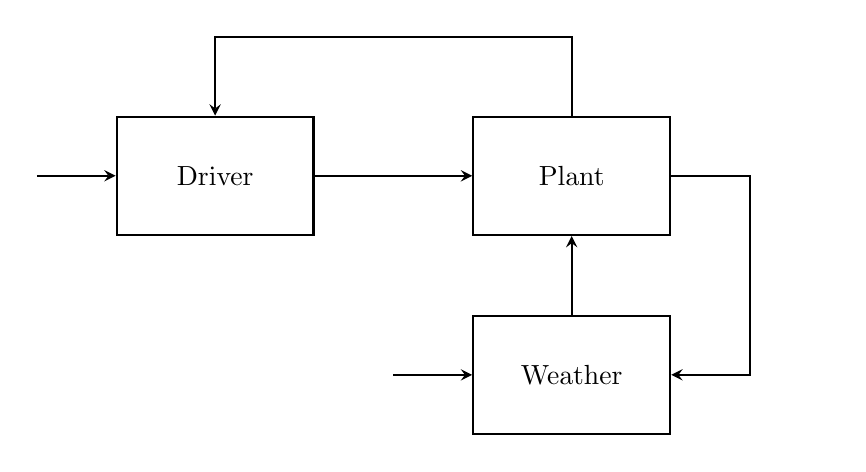
\begin{tikzpicture}
	
	% Blocks
	\matrix[column sep=1cm, row sep=1cm]{
	%first row
	&
	\coordinate (c12); &
	&
	\coordinate (c14); &
	&
	\\
	%second row
	\coordinate (c21); &
	\node[block] (driver) {Driver}; &
	&
	\node[block] (plant) {Plant}; &
	\coordinate (c25); &
	\\
	%third row
	&
	&
	\coordinate (c33); &
	\node[block] (weather) {Weather}; &
	\coordinate (c35); &
	\\
	};

	% Arrows
	\draw[arrow] (c21) -- (driver);
	\draw[arrow] (c33) -- (weather);
	\draw[arrow] (driver) -- (plant);
	\draw[arrow] (weather) -- (plant);
	\draw[arrow] (plant) -- (c25) -- (c35) -- (weather);
	\draw[arrow] (plant) -- (c14) -- (c12) -- (driver);
	

\end{tikzpicture}